% Options for packages loaded elsewhere
\PassOptionsToPackage{unicode}{hyperref}
\PassOptionsToPackage{hyphens}{url}
%
\documentclass[
]{book}
\usepackage{amsmath,amssymb}
\usepackage{iftex}
\ifPDFTeX
  \usepackage[T1]{fontenc}
  \usepackage[utf8]{inputenc}
  \usepackage{textcomp} % provide euro and other symbols
\else % if luatex or xetex
  \usepackage{unicode-math} % this also loads fontspec
  \defaultfontfeatures{Scale=MatchLowercase}
  \defaultfontfeatures[\rmfamily]{Ligatures=TeX,Scale=1}
\fi
\usepackage{lmodern}
\ifPDFTeX\else
  % xetex/luatex font selection
\fi
% Use upquote if available, for straight quotes in verbatim environments
\IfFileExists{upquote.sty}{\usepackage{upquote}}{}
\IfFileExists{microtype.sty}{% use microtype if available
  \usepackage[]{microtype}
  \UseMicrotypeSet[protrusion]{basicmath} % disable protrusion for tt fonts
}{}
\makeatletter
\@ifundefined{KOMAClassName}{% if non-KOMA class
  \IfFileExists{parskip.sty}{%
    \usepackage{parskip}
  }{% else
    \setlength{\parindent}{0pt}
    \setlength{\parskip}{6pt plus 2pt minus 1pt}}
}{% if KOMA class
  \KOMAoptions{parskip=half}}
\makeatother
\usepackage{xcolor}
\usepackage{color}
\usepackage{fancyvrb}
\newcommand{\VerbBar}{|}
\newcommand{\VERB}{\Verb[commandchars=\\\{\}]}
\DefineVerbatimEnvironment{Highlighting}{Verbatim}{commandchars=\\\{\}}
% Add ',fontsize=\small' for more characters per line
\usepackage{framed}
\definecolor{shadecolor}{RGB}{248,248,248}
\newenvironment{Shaded}{\begin{snugshade}}{\end{snugshade}}
\newcommand{\AlertTok}[1]{\textcolor[rgb]{0.94,0.16,0.16}{#1}}
\newcommand{\AnnotationTok}[1]{\textcolor[rgb]{0.56,0.35,0.01}{\textbf{\textit{#1}}}}
\newcommand{\AttributeTok}[1]{\textcolor[rgb]{0.13,0.29,0.53}{#1}}
\newcommand{\BaseNTok}[1]{\textcolor[rgb]{0.00,0.00,0.81}{#1}}
\newcommand{\BuiltInTok}[1]{#1}
\newcommand{\CharTok}[1]{\textcolor[rgb]{0.31,0.60,0.02}{#1}}
\newcommand{\CommentTok}[1]{\textcolor[rgb]{0.56,0.35,0.01}{\textit{#1}}}
\newcommand{\CommentVarTok}[1]{\textcolor[rgb]{0.56,0.35,0.01}{\textbf{\textit{#1}}}}
\newcommand{\ConstantTok}[1]{\textcolor[rgb]{0.56,0.35,0.01}{#1}}
\newcommand{\ControlFlowTok}[1]{\textcolor[rgb]{0.13,0.29,0.53}{\textbf{#1}}}
\newcommand{\DataTypeTok}[1]{\textcolor[rgb]{0.13,0.29,0.53}{#1}}
\newcommand{\DecValTok}[1]{\textcolor[rgb]{0.00,0.00,0.81}{#1}}
\newcommand{\DocumentationTok}[1]{\textcolor[rgb]{0.56,0.35,0.01}{\textbf{\textit{#1}}}}
\newcommand{\ErrorTok}[1]{\textcolor[rgb]{0.64,0.00,0.00}{\textbf{#1}}}
\newcommand{\ExtensionTok}[1]{#1}
\newcommand{\FloatTok}[1]{\textcolor[rgb]{0.00,0.00,0.81}{#1}}
\newcommand{\FunctionTok}[1]{\textcolor[rgb]{0.13,0.29,0.53}{\textbf{#1}}}
\newcommand{\ImportTok}[1]{#1}
\newcommand{\InformationTok}[1]{\textcolor[rgb]{0.56,0.35,0.01}{\textbf{\textit{#1}}}}
\newcommand{\KeywordTok}[1]{\textcolor[rgb]{0.13,0.29,0.53}{\textbf{#1}}}
\newcommand{\NormalTok}[1]{#1}
\newcommand{\OperatorTok}[1]{\textcolor[rgb]{0.81,0.36,0.00}{\textbf{#1}}}
\newcommand{\OtherTok}[1]{\textcolor[rgb]{0.56,0.35,0.01}{#1}}
\newcommand{\PreprocessorTok}[1]{\textcolor[rgb]{0.56,0.35,0.01}{\textit{#1}}}
\newcommand{\RegionMarkerTok}[1]{#1}
\newcommand{\SpecialCharTok}[1]{\textcolor[rgb]{0.81,0.36,0.00}{\textbf{#1}}}
\newcommand{\SpecialStringTok}[1]{\textcolor[rgb]{0.31,0.60,0.02}{#1}}
\newcommand{\StringTok}[1]{\textcolor[rgb]{0.31,0.60,0.02}{#1}}
\newcommand{\VariableTok}[1]{\textcolor[rgb]{0.00,0.00,0.00}{#1}}
\newcommand{\VerbatimStringTok}[1]{\textcolor[rgb]{0.31,0.60,0.02}{#1}}
\newcommand{\WarningTok}[1]{\textcolor[rgb]{0.56,0.35,0.01}{\textbf{\textit{#1}}}}
\usepackage{longtable,booktabs,array}
\usepackage{calc} % for calculating minipage widths
% Correct order of tables after \paragraph or \subparagraph
\usepackage{etoolbox}
\makeatletter
\patchcmd\longtable{\par}{\if@noskipsec\mbox{}\fi\par}{}{}
\makeatother
% Allow footnotes in longtable head/foot
\IfFileExists{footnotehyper.sty}{\usepackage{footnotehyper}}{\usepackage{footnote}}
\makesavenoteenv{longtable}
\usepackage{graphicx}
\makeatletter
\def\maxwidth{\ifdim\Gin@nat@width>\linewidth\linewidth\else\Gin@nat@width\fi}
\def\maxheight{\ifdim\Gin@nat@height>\textheight\textheight\else\Gin@nat@height\fi}
\makeatother
% Scale images if necessary, so that they will not overflow the page
% margins by default, and it is still possible to overwrite the defaults
% using explicit options in \includegraphics[width, height, ...]{}
\setkeys{Gin}{width=\maxwidth,height=\maxheight,keepaspectratio}
% Set default figure placement to htbp
\makeatletter
\def\fps@figure{htbp}
\makeatother
\setlength{\emergencystretch}{3em} % prevent overfull lines
\providecommand{\tightlist}{%
  \setlength{\itemsep}{0pt}\setlength{\parskip}{0pt}}
\setcounter{secnumdepth}{5}
\usepackage{booktabs}
\ifLuaTeX
  \usepackage{selnolig}  % disable illegal ligatures
\fi
\usepackage[]{natbib}
\bibliographystyle{plainnat}
\usepackage{bookmark}
\IfFileExists{xurl.sty}{\usepackage{xurl}}{} % add URL line breaks if available
\urlstyle{same}
\hypersetup{
  pdftitle={PSYNETS: R Essentials},
  pdfauthor={The PSYNETS Team},
  hidelinks,
  pdfcreator={LaTeX via pandoc}}

\title{PSYNETS: R Essentials}
\author{The PSYNETS Team}
\date{2024-10-23}

\begin{document}
\maketitle

{
\setcounter{tocdepth}{1}
\tableofcontents
}
\chapter{Introduction}\label{introduction}

This book is designed for participants of the PSYNETS workshop to help them get acquainted with the basic functionalities of R and the R packages used throughout the sessions. It has been compiled based on the most frequently asked questions and challenges that participants have encountered during previous workshops. While not a comprehensive guide to R for network psychometrics, it serves as a quick reference to help you get started with R and the specific packages used in the workshop. The primary focus is on installing packages, loading data from various formats, and understanding the unique features of each packages covered in the course. Whenever you have a technical question about R, we recommend consulting this book first.

\section{Structure of the book}\label{structure-of-the-book}

This book is structured as follows\ldots{}

\chapter{Introduction to R for Absolute Beginners}\label{introduction-to-r-for-absolute-beginners}

Welcome to R! This guide is designed to help absolute beginners get started with R, a powerful tool for statistical computing and data visualization. R can seem overwhelming at first, but this introduction will walk you through the basics, step by step. If you are already familiar with R, feel free to skip this section.

\section{What is R?}\label{what-is-r}

R is a programming language and software environment specifically designed for statistical analysis and data visualization. It is widely used by data scientists, statisticians, and researchers.

\section{Getting Started with R}\label{getting-started-with-r}

\subsection{Installing R and RStudio}\label{installing-r-and-rstudio}

To use R, you will need two things:
1. \textbf{R}: Download and install it from \href{https://cran.r-project.org/}{CRAN}.
2. \textbf{RStudio}: A user-friendly interface for R, which you can download from \href{https://posit.co/download/rstudio-desktop/}{RStudio's website}.

\subsection{RStudio Interface}\label{rstudio-interface}

When you open RStudio, you'll see four main panels:
- \textbf{Source/Script Editor}: Write and save your R code here.
- \textbf{Console}: Run code directly and see the output.
- \textbf{Environment/History}: See your data and objects.
- \textbf{Files/Plots/Packages/Help}: Access files, view plots, manage packages, and get help. you can easily load data sets using this option.

\section{Basic Syntax in R}\label{basic-syntax-in-r}

\subsection{Running Code}\label{running-code}

You can run code directly in the console or write it in the script editor and press \texttt{Ctrl\ +\ Enter} (or \texttt{Cmd\ +\ Enter} on a Mac) to run it. We always suggest you do the later, that way your code is saved.

\subsection{Basic Calculations}\label{basic-calculations}

At its simplest, R can be used as a calculator. For example:

\begin{Shaded}
\begin{Highlighting}[]
\DecValTok{1} \SpecialCharTok{+} \DecValTok{1}
\DecValTok{5} \SpecialCharTok{*} \DecValTok{3}
\DecValTok{10} \SpecialCharTok{/} \DecValTok{2}
\DecValTok{2}\SpecialCharTok{\^{}}\DecValTok{3}
\end{Highlighting}
\end{Shaded}

\subsection{Variables}\label{variables}

You can store values in \textbf{variables} or as they sometimes called \textbf{objects}. A variable is like a box that holds data.

\begin{Shaded}
\begin{Highlighting}[]
\NormalTok{x }\OtherTok{\textless{}{-}} \DecValTok{5}
\NormalTok{y }\OtherTok{\textless{}{-}} \DecValTok{10}
\NormalTok{sum }\OtherTok{\textless{}{-}}\NormalTok{ x }\SpecialCharTok{+}\NormalTok{ y}
\NormalTok{sum}
\end{Highlighting}
\end{Shaded}

\subsection{Data Types}\label{data-types}

R has several basic data types:

\begin{itemize}
\tightlist
\item
  Numeric: Numbers like 42 or 3.14.
\item
  Character: Text or strings like ``Hello''.
\item
  Logical: \texttt{TRUE} or \texttt{FALSE}.
\end{itemize}

\begin{Shaded}
\begin{Highlighting}[]
\NormalTok{num\_var }\OtherTok{\textless{}{-}} \DecValTok{42}  \CommentTok{\# numeric}
\NormalTok{char\_var }\OtherTok{\textless{}{-}} \StringTok{"Hello, R!"}  \CommentTok{\# string}
\NormalTok{log\_var }\OtherTok{\textless{}{-}} \ConstantTok{TRUE} \CommentTok{\# logical }
\end{Highlighting}
\end{Shaded}

\subsection{Functions}\label{functions}

A function is a piece of code that performs a specific task. For example, \texttt{sqrt()} calculates the square root:

\begin{Shaded}
\begin{Highlighting}[]
\FunctionTok{sqrt}\NormalTok{(}\DecValTok{16}\NormalTok{)}
\end{Highlighting}
\end{Shaded}

There are many in-built functions in R, and you can also create your own functions. And of course, as you will see in the rest of the chapters, many of the functionalities you will use come from packages, which can be installed and loaded follows:

\begin{Shaded}
\begin{Highlighting}[]
\FunctionTok{install.packages}\NormalTok{(}\StringTok{"package\_name"}\NormalTok{)}
\FunctionTok{library}\NormalTok{(package\_name)}
\end{Highlighting}
\end{Shaded}

\section{Working with Data}\label{working-with-data}

\subsection{Vectors}\label{vectors}

A vector is a sequence of data elements of the same basic type. You can create a vector using the \texttt{c()} function:

\begin{Shaded}
\begin{Highlighting}[]
\NormalTok{my\_vector }\OtherTok{\textless{}{-}} \FunctionTok{c}\NormalTok{(}\DecValTok{1}\NormalTok{, }\DecValTok{2}\NormalTok{, }\DecValTok{3}\NormalTok{, }\DecValTok{4}\NormalTok{, }\DecValTok{5}\NormalTok{)}
\NormalTok{my\_vector}
\end{Highlighting}
\end{Shaded}

\subsection{Data Frames}\label{data-frames}

A data frame is a table-like data structure (i.e., a spreadsheet) that stores data. You can create a data frame using the
\texttt{data.frame()} function:

\begin{Shaded}
\begin{Highlighting}[]
\NormalTok{my\_data }\OtherTok{\textless{}{-}} \FunctionTok{data.frame}\NormalTok{(}
  \AttributeTok{Name =} \FunctionTok{c}\NormalTok{(}\StringTok{"A"}\NormalTok{, }\StringTok{"B"}\NormalTok{, }\StringTok{"C"}\NormalTok{),}
  \AttributeTok{Age =} \FunctionTok{c}\NormalTok{(}\DecValTok{25}\NormalTok{, }\DecValTok{30}\NormalTok{, }\DecValTok{35}\NormalTok{),}
  \AttributeTok{Height =} \FunctionTok{c}\NormalTok{(}\DecValTok{175}\NormalTok{, }\DecValTok{182}\NormalTok{, }\DecValTok{168}\NormalTok{)}
\NormalTok{)}
\NormalTok{my\_data}
\end{Highlighting}
\end{Shaded}

\begin{verbatim}
##   Name Age Height
## 1    A  25    175
## 2    B  30    182
## 3    C  35    168
\end{verbatim}

\section{Loading Data into R}\label{loading-data-into-r}

R can read data from various file formats, as already mentioned, you can also use the file tab for this. Here are some examples of how this if formally done through the console, for some common file formats. Before we start, make sure to set your working directory to the location where your data is stored. You can set your working directory using the \texttt{setwd()} function. Alternatively, you can use the \texttt{here} package to set your working directory to the location of your R script. You can also navigate on top of R studio to the session tab and set your working directory from there. Finally you can use the keyboard shortcut \texttt{Ctrl\ +\ Shift\ +\ H} to set your working directory.

\subsection{Reading a CSV file}\label{reading-a-csv-file}

\begin{Shaded}
\begin{Highlighting}[]
\CommentTok{\# Make sure the \textquotesingle{}data.csv\textquotesingle{} file is in your working directory}
\NormalTok{my\_data }\OtherTok{\textless{}{-}} \FunctionTok{read.csv}\NormalTok{(}\StringTok{"data.csv"}\NormalTok{)}
\FunctionTok{head}\NormalTok{(my\_data)}
\end{Highlighting}
\end{Shaded}

\subsection{Reading an Excel File}\label{reading-an-excel-file}

\begin{Shaded}
\begin{Highlighting}[]
\CommentTok{\# Install the readxl package if you haven\textquotesingle{}t already}
\CommentTok{\#install.packages("readxl")}
\FunctionTok{library}\NormalTok{(readxl)}

\CommentTok{\# Reading an Excel file}
\NormalTok{my\_data }\OtherTok{\textless{}{-}} \FunctionTok{read\_excel}\NormalTok{(}\StringTok{"data.xlsx"}\NormalTok{, }\AttributeTok{sheet =} \DecValTok{1}\NormalTok{)}
\FunctionTok{head}\NormalTok{(my\_data)}
\end{Highlighting}
\end{Shaded}

\subsection{Reading Data from R's Built-in Datasets}\label{reading-data-from-rs-built-in-datasets}

Many R packages come with built-in datasets that you can use to practice. For example, the \texttt{mtcars} dataset is built into R:

\begin{Shaded}
\begin{Highlighting}[]
\CommentTok{\# Load the \textquotesingle{}mtcars\textquotesingle{} dataset}
\FunctionTok{data}\NormalTok{(mtcars)}
\FunctionTok{head}\NormalTok{(mtcars)}
\end{Highlighting}
\end{Shaded}

\begin{verbatim}
##                    mpg cyl disp  hp drat    wt  qsec vs am gear carb
## Mazda RX4         21.0   6  160 110 3.90 2.620 16.46  0  1    4    4
## Mazda RX4 Wag     21.0   6  160 110 3.90 2.875 17.02  0  1    4    4
## Datsun 710        22.8   4  108  93 3.85 2.320 18.61  1  1    4    1
## Hornet 4 Drive    21.4   6  258 110 3.08 3.215 19.44  1  0    3    1
## Hornet Sportabout 18.7   8  360 175 3.15 3.440 17.02  0  0    3    2
## Valiant           18.1   6  225 105 2.76 3.460 20.22  1  0    3    1
\end{verbatim}

\section{Doing a statistical analysis}\label{doing-a-statistical-analysis}

R is a powerful tool for statistical analysis. You can perform a wide range of statistical tests and analyses using R. Here is an example of how to perform a simple t-test.

\subsection{T-Test}\label{t-test}

\begin{Shaded}
\begin{Highlighting}[]
\CommentTok{\# Subset the data into two groups}
\NormalTok{auto }\OtherTok{\textless{}{-}}\NormalTok{ mtcars}\SpecialCharTok{$}\NormalTok{mpg[mtcars}\SpecialCharTok{$}\NormalTok{am }\SpecialCharTok{==} \DecValTok{0}\NormalTok{]  }\CommentTok{\# Automatic cars}
\NormalTok{manual }\OtherTok{\textless{}{-}}\NormalTok{ mtcars}\SpecialCharTok{$}\NormalTok{mpg[mtcars}\SpecialCharTok{$}\NormalTok{am }\SpecialCharTok{==} \DecValTok{1}\NormalTok{]  }\CommentTok{\# Manual cars}

\CommentTok{\# Perform a t{-}test}
\NormalTok{t\_test\_result }\OtherTok{\textless{}{-}} \FunctionTok{t.test}\NormalTok{(auto, manual)}
\NormalTok{t\_test\_result}
\end{Highlighting}
\end{Shaded}

\begin{verbatim}
## 
##  Welch Two Sample t-test
## 
## data:  auto and manual
## t = -3.7671, df = 18.332, p-value = 0.001374
## alternative hypothesis: true difference in means is not equal to 0
## 95 percent confidence interval:
##  -11.280194  -3.209684
## sample estimates:
## mean of x mean of y 
##  17.14737  24.39231
\end{verbatim}

\subsection{Visualizing data}\label{visualizing-data}

R is also great for data visualization. You can create a wide range of plots and graphs using R. Here is an example of how to create a boxlot. R has in built functions for many types of plots, and you can also use the \texttt{ggplot2} package for more advanced plots.

\begin{Shaded}
\begin{Highlighting}[]
\FunctionTok{boxplot}\NormalTok{(mpg }\SpecialCharTok{\textasciitilde{}}\NormalTok{ am, }\AttributeTok{data =}\NormalTok{ mtcars,}
        \AttributeTok{main =} \StringTok{"Miles Per Gallon (mpg) by Transmission Type"}\NormalTok{,}
        \AttributeTok{xlab =} \StringTok{"Transmission (0 = Automatic, 1 = Manual)"}\NormalTok{,}
        \AttributeTok{ylab =} \StringTok{"Miles Per Gallon (mpg)"}\NormalTok{)}
\end{Highlighting}
\end{Shaded}

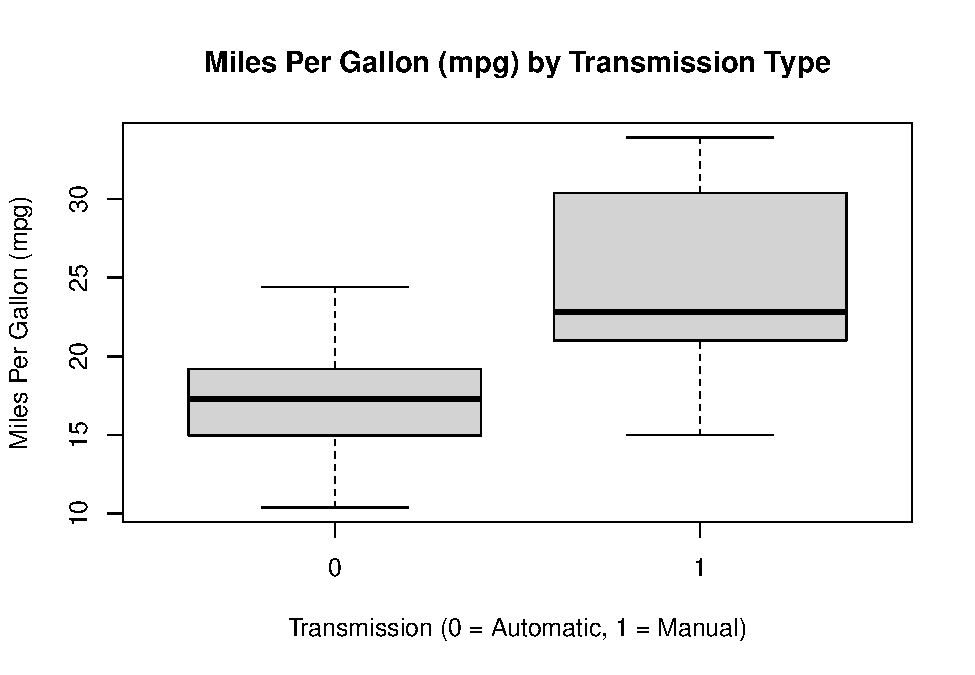
\includegraphics{_main_files/figure-latex/unnamed-chunk-12-1.pdf}

\section{Additional Resources}\label{additional-resources}

This introduction is just the tip of the iceberg. R is a vast and powerful tool with a steep learning curve. Here are some additional resources to help you continue your journey with R:

\begin{itemize}
\tightlist
\item
  \href{https://r4ds.had.co.nz/}{R for Data Science}: A comprehensive guide to data science with R.
\item
  \href{https://www.rstudio.com/resources/cheatsheets/}{RStudio Cheatsheets}: Handy cheatsheets for various R topics.
\item
  \href{https://stackoverflow.com/}{Stack Overflow}: A great place to ask questions and find answers about R.
\item
  \href{https://www.rdocumentation.org/}{R Documentation}: Official documentation for R packages.
\end{itemize}

\section{Conclusion}\label{conclusion}

Congratulations! You've completed the introduction to R. We hope this guide has given you a solid foundation to start exploring R on your own.

\chapter{Package 1}\label{package-1}

  \bibliography{book.bib,packages.bib}

\end{document}
